% Setup - do not change
\documentclass[11pt]{article}
\usepackage[top=0.9in, left=0.9in, bottom=0.9in, right=0.9in]{geometry} 
\usepackage{parskip}
\usepackage{booktabs}
\usepackage[T1]{fontenc}
\usepackage{float}

\usepackage[english]{babel}
\usepackage[utf8]{inputenc}
\usepackage{amsmath,amsthm,amssymb,graphicx,pdfpages,lipsum,hyperref}
\usepackage[none]{hyphenat}
\usepackage{csquotes}
\usepackage{caption}
\usepackage{subcaption}



\setlength\parindent{0pt}
%%%%%%%%%%%%%%%%%%%%%%%%%%%%%%%%%%%%%%%%%%%%%%%%%%%%%%%%%%%%%%%%%%%
% add other packages here if required

%% Bibliography are specified in this file. You can also choose inline bib style if you want to. But make sure your citation style is consistent (and proper)
% For more details on citation: https://library.unimelb.edu.au/recite
\usepackage[sorting = none]{biblatex}
\addbibresource{references.bib}

%%%%%%%%%%%%%%%%%%%%%%%%%%%%%%%%%%%%%%%%%%%%%%%%%%%%%%%%%%%%%%%%%%% the '%' symbol denotes comments

% Begin document creation
\title{\textbf{Modelling Airport High Volume For-Hire Vehicle Demand Using Hourly Flight Data}}
\author{
Saurabh Jhanjee \\
Student ID: 1071081 \\
%% Replace the link with your github repo
% 1. Remember to escape underscore (\_) in the link.
% 2. Remember to include the commit you want to submit in the link
\href{https://github.com/MAST30034-Applied-Data-Science/mast30034-project-1-Shrub24/commit/03eb9c8c98d67463c8eef1748ecac35c523aac81}{Github repo with commit}
}

\begin{document}
\maketitle

\section{Introduction}
% Link to a 30 min tutorial if you require revision: https://www.overleaf.com/learn/latex/Learn_LaTeX_in_30_minutes

High volume for-hire vehicle services such as Uber and Lyft dominate the private transportation industry around the world. One main competitive advantage these companies have over traditional taxi services is the algorithms they use to model demand using the vast amounts of data they have access to and thus are able to successfully employ multiple-pricing strategies (surge pricing, fees etc.) to maximise profits. Airport surge pricing is a well-known strategy used by these services as airports are areas of anomalously high demand driven by external factors relating to flight and passenger volume. In this paper, we attempt to model this external factor of demand using TLC New York datasets \cite{thebigtaxidataset} paired with hourly flight data from ASPM \cite{2021aspmflightdata}. We aim to identify the differences in hourly volume distribution in airport TLC zones (compared to other TLC zones across NYC) using hypothesis tests and form a more robust model for demand for trips from and to airport TLC zones by including and measuring the effect of the ASPM flight data using a linear regression (ElasticNet) based model.

We use the FHVHV dataset as it is most relevant to our research, as surge pricing is most prevalent in high volume services and thus airport volume modelling is most valuable for such trips. We study flight volume data from the ASPM dataset, particularly departures and arrival numbers by hour and facility. We aggregate hourly FHV counts by facility (using location IDs to identify airport trips), and include temporal variables such as day to account for seasonal trends. Our target audience is both high volume FHV services (such as Uber, Lyft etc.) who may use this model to inform surge pricing and their drivers who may use this to better allocate supply, as well as customers (and customer facing agencies) who may seek to minimise transportation costs by avoiding high volume times. We select 01/2021-07/2021 as our dataset to analyse and train our model, being the earliest available complete dataset for fhvhv. We select 02/2022-04/2022 as our testing dataset to evaluate if our models generalise well to recent (and future) periods.


% You can have \section{}, \subsection{}, and \subsubsection{}


\section{Data Processing and Analysis}
\subsection{Dataset}
In this analysis, we rely primarily on 2 datasets. Firstly, the NYC Taxi \& Limousine Commission (NYCTLC) For-Hire Vehicle High Volume (FHVHV) dataset \cite{thebigtaxidataset}, which records trip details for for-hire vehicle rides commissioned through a "High Volume" service (such as Uber, Lyft etc). Secondly, we use the Federal Aviation Administration (FAA) Aviation System Performance Metrics (ASPM) dataset \cite{2021aspmflightdata}, which contains metrics about flight departures and arrivals at airports across the USA, at an hourly level.
\subsection{High-Level Preprocessing (Data Extraction and Aggregation)}
\begin{enumerate} 
    \item First we begin preprocessing by removing irrelevant data from the TLC dataset. As we plan analyse ride volume by hour, we are most interested in counting "valid rides", and thus we must exclude any invalid rides. For the purposes of our analysis, this entails culling any records with a negative fare, as these records do not represent actual rides, rather charge-backs of preceding rides. Apart from this, we do not exclude any outlying data from our analysis, as outlying column values (apart from datetime values, which will automatically be excluded on our subsequent join with the flight dataset) will not affect our analysis and are not a sufficient indicator of an "invalid ride" (eg. an outlying column value does not sufficiently invalidate a whole record from being counted and does not adversely effect our analysis). We must also filter our data to only contain rides to or from airports using the relevant TLC zones (1, 132, 138), generating two separate datasets for airport pickups and dropoffs respectively.
    \item Next we must obtain the relevant statistics for our analysis. This was done by first grouping records by requesting "airport" "hour" and "date", then aggregating the ride counts for each group. We also generate columns representing the subsequent and preceding 5 hours and dates corresponding to each ride count to allow temporally shifted analysis (5 hours was chosen as most international flights recommend a 3 hour early arrival, and we assume a maximal expected travel time of 2 hours). These new columns will allow us to iteratively join with the flight dataset and obtain departure and arrival data spanning the preceding 5 hours and following 5 hours as features for our analysis. 
    % use \item to create more points
\end{enumerate}
\subsection{Feature Selection}
Now that we have aggregated and generated a number of relevant features to predict ride count, we must now choose which of these are relevant to the two problems presented.
\subsubsection{Airport Dropoffs Features}
We begin by examining the relevant categorical features such as day and facility using ANOVA. We do not consider hour, date and month as these would require a much larger number of indicator variables to model and may encourage overfitting due to overparameterisation. Furthermore, they may serve to associate the data with a given timestamp and thus reduce the generalisability of the model to other years. Hour is specifically not considered as daily time information is already somewhat encoded within flight data.

\begin{table}[h!]
\centering
\caption{One way ANOVA - Day}
\label{tbl:anova_day}
\begin{tabular}{lrrrr}
\toprule
{} &        sum\_sq &       df &          F &        PR(>F) \\
\midrule
C(Day)   &  6.272285e+06 &      6.0 &  38.286814 &  2.718924e-46 \\
Residual &  3.035925e+08 &  11119.0 &         &            \\
\bottomrule
\end{tabular}
\end{table}

\begin{table}[H]
\centering
\caption{One way ANOVA - Facility}
\label{tbl:anova_facility}
\begin{tabular}{lrrrr}
\toprule
{} &        sum\_sq &       df &            F &  PR(>F) \\
\midrule
C(Facility) &  6.338480e+07 &      2.0 &  1430.195648 &     0.0 \\
Residual    &  2.464800e+08 &  11123.0 &           &      \\
\bottomrule
\end{tabular}
\end{table}

\begin{table}[H]
\centering
\caption{Two way ANOVA with interaction - Day \& Facility}
\label{tbl:anova_interaction}
\begin{tabular}{lrrrr}
\toprule
{} &        sum\_sq &       df &            F &        PR(>F) \\
\midrule
C(Facility)        &  6.385527e+07 &      2.0 &  1492.334127 &  0.000000e+00 \\
C(Day)             &  6.742758e+06 &      6.0 &    52.527365 &  3.904188e-64 \\
C(Facility):C(Day) &  2.152066e+06 &     12.0 &     8.382503 &  5.128350e-16 \\
Residual           &  2.375851e+08 &  11105.0 &           &            \\
\bottomrule
\end{tabular}
\end{table}



For airport dropoffs, intuitively we except departures in the next few hours to have the largest explanatory impact on ride counts (as people will be dropped off at the airport for their future departures). In order to ascertain which other features may be correlated to ride counts, we can use Pearson's correlation coefficient.

\begin{figure}[H]
    \centering
    \caption{Correlation between time shifted arrival/departure features and dropoff count}
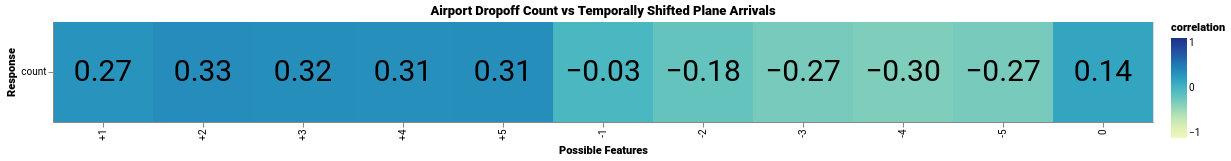
\includegraphics[width=1\textwidth]{plots/dropoff_arrival_corr.png}
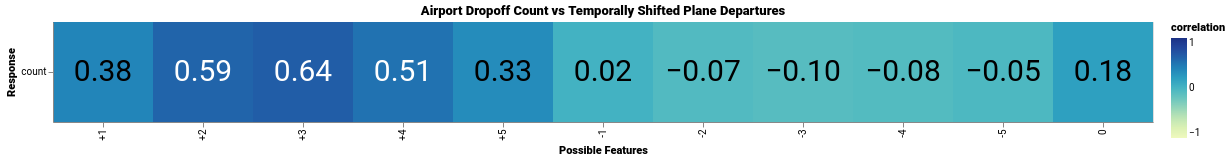
\includegraphics[width=1\textwidth]{plots/dropoff_departure_corr.png}
\end{figure}

As expected, future departure features are most heavily correlated to our response. However, future arrivals seem to also similarly be positively correlated to counts. Furthermore, past arrivals seem to have a somewhat notable negative correlation to counts. In rationalising these results, it is possible that these correlations are merely the result of being heavily collinear with future departures, particularly for the future arrivals columns (as these are obviously temporally linked).

\begin{figure}[h!]
    \centering
    \caption{Correlation between pairs of time shifted arrivals vs departures}
    \label{fig:corr_pairs}
    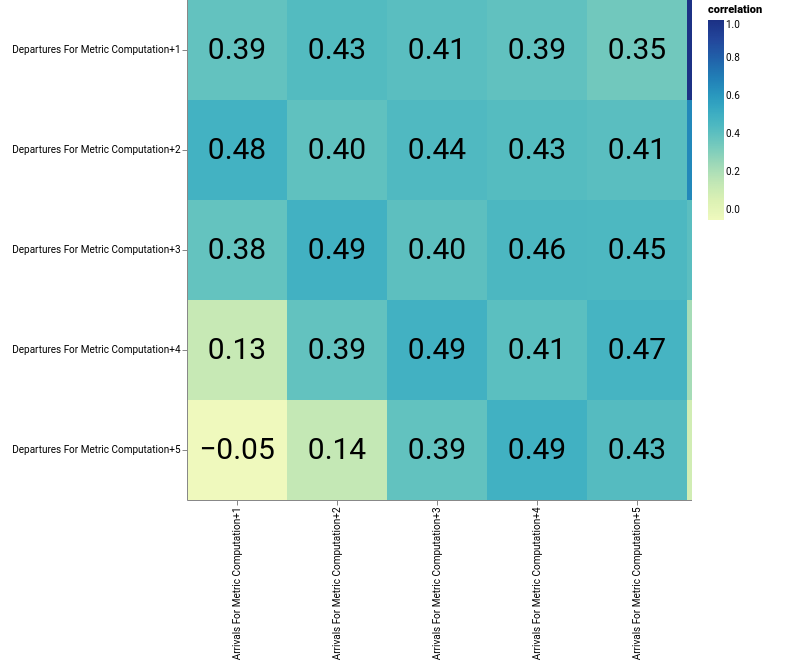
\includegraphics[width=0.5\textwidth]{plots/arrival_departure_time_correlation.png}
\end{figure}

This correlation matrix \ref{fig:corr_pairs} demonstrates the correlation between pairs of arrivals/departure by temporal difference. Note that this mostly generalises to past arrivals/departures as the feature values are identical (just shifted).

On the other hand, it is plausible that past arrivals may actually have a negative impact on ride volumes, as past arrivals may be an indicator of a lower available supply of vehicles (as they may be busy picking people up), and thus lesser drop off volume. 

Hence, as per the above, we choose departures up to 5 hours into the future, and arrivals up to 5 hours in the past as our relevant flight data columns. Furthermore, we also include facility and day indicator variables (dummy variables) as per the ANOVA analysis \ref{tbl:anova_day}\ref{tbl:anova_facility}.
\subsubsection{Airport Pickup Features}

Conversely, for airport pickups, we intuitively expect past arrivals to have the greatest correlation with ride counts. We once again use Pearson's correlation coefficient.
\begin{figure}[h!]
    \centering
    \caption{Correlation between time shifted arrival/departure features and pickup count}
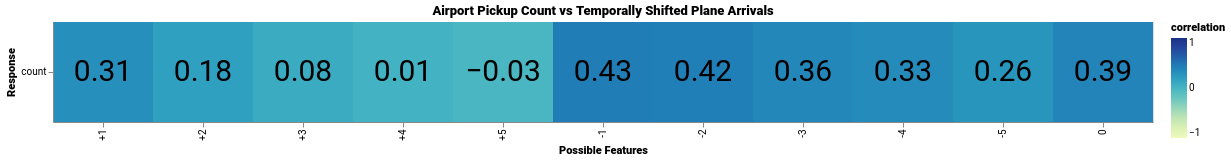
\includegraphics[width=1\textwidth]{plots/pickup_arrival_corr.png}
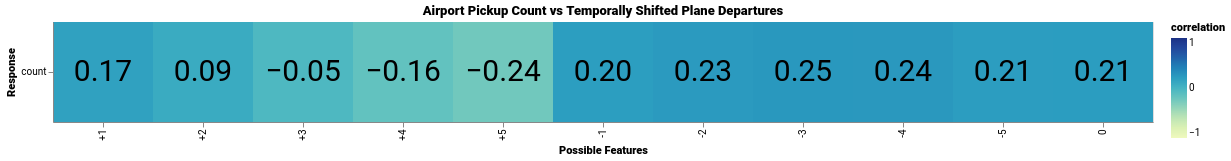
\includegraphics[width=1\textwidth]{plots/pickup_departure_corr.png}

\end{figure}

Once again, as expected past arrivals has the heaviest correlation with our response. In this case we also observe a non-trivial (albeit lesser) correlation with certain future departure variables, as well as a similarly high correlation with past departures. Again, the response's correlation with past departures can be explained by a high correlation between future departures and arrivals (of which arrivals is clearly and intuitively more explanatory). In this case we have also chosen to include the future departures, although the intuition for such is less clear than in the former case. It could possibly be due to drivers being more likely to accept rides when there is a high demand for dropoffs in the future (ie more departures), as to return to their origin airport. We also include day and facility columns. The ANOVA analysis here for the sake of brevity, it follows similar methods and results as per \ref{tbl:anova_day}\ref{tbl:anova_facility}.

\section{Models}
\subsection{Elastic Net Least Squares Regression (OLS)}
We begin with a simple regression model, using Elastic Net as our model. We standarise our data to the standard normal distribution in order to work well with the regularisation implemented by Elastic Net. We use the below pipeline \ref{fig:elasticnet_pipeline} to process and fit our data, as well as choose our hyperparameters using a cross-validated (k=5) grid search on the training data. We create "dummy" indicator variables for day and facility in order to include these in our OLS model.
\begin{figure}[h!]
    \centering
    \caption{Elastic Net Pipeline}
    \label{fig:elasticnet_pipeline}
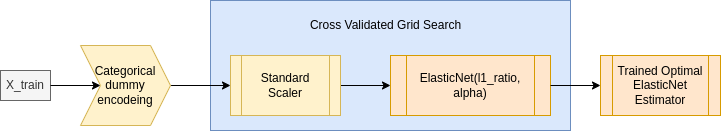
\includegraphics[width=1\textwidth]{plots/elasticnet_pipeline.png}
\end{figure}


\begin{figure}[H]

\captionof{table}{CV Grid Search Avg. $R^2$ scores across folds for l1 ratio and $\alpha$}
\[
    Pickups
  \begin{array}{cc|ccccc}
    &\multicolumn{1}{c}{} & \multicolumn{5}{c}{\text{l1 ratio}} \\
    && .1 & \textbf{.5} & .7 & .9 & 1 \\
    \cline{2-7}
    & \textbf{.1} & .728 & \textbf{.729} & .728 & .728 & .727 \\
    \smash{\rotatebox[origin=c]{90}{\text{$\alpha$}}} & 1 & .641 & .690 & .713 & .727 & .727 \\
    & 10 & .175 & .286 & .388 & .576 & .710
  \end{array}
  \qquad
  Dropoffs
  \begin{array}{cc|ccccc}
    &\multicolumn{1}{c}{} & \multicolumn{5}{c}{\text{l1 ratio}} \\
    && \textbf{.1} & .5 & .7 & .9 & 1 \\
    \cline{2-7}
    & \textbf{.1} & \textbf{.681} & .681 & .680 & .679 & .678 \\
    \smash{\rotatebox[origin=c]{90}{\text{$\alpha$}}} & 1 & .547 & .620 & .655 & .679 & .679 \\
    & 10 & .023 & .118 & .215 & .425 & .619
  \end{array}
\]


\end{figure}


\begin{figure}[H]
    \centering
    \caption{Dropoffs Performance Visualisation on a subset of test data by facility}
    \label{fig:dropoffsperformance}
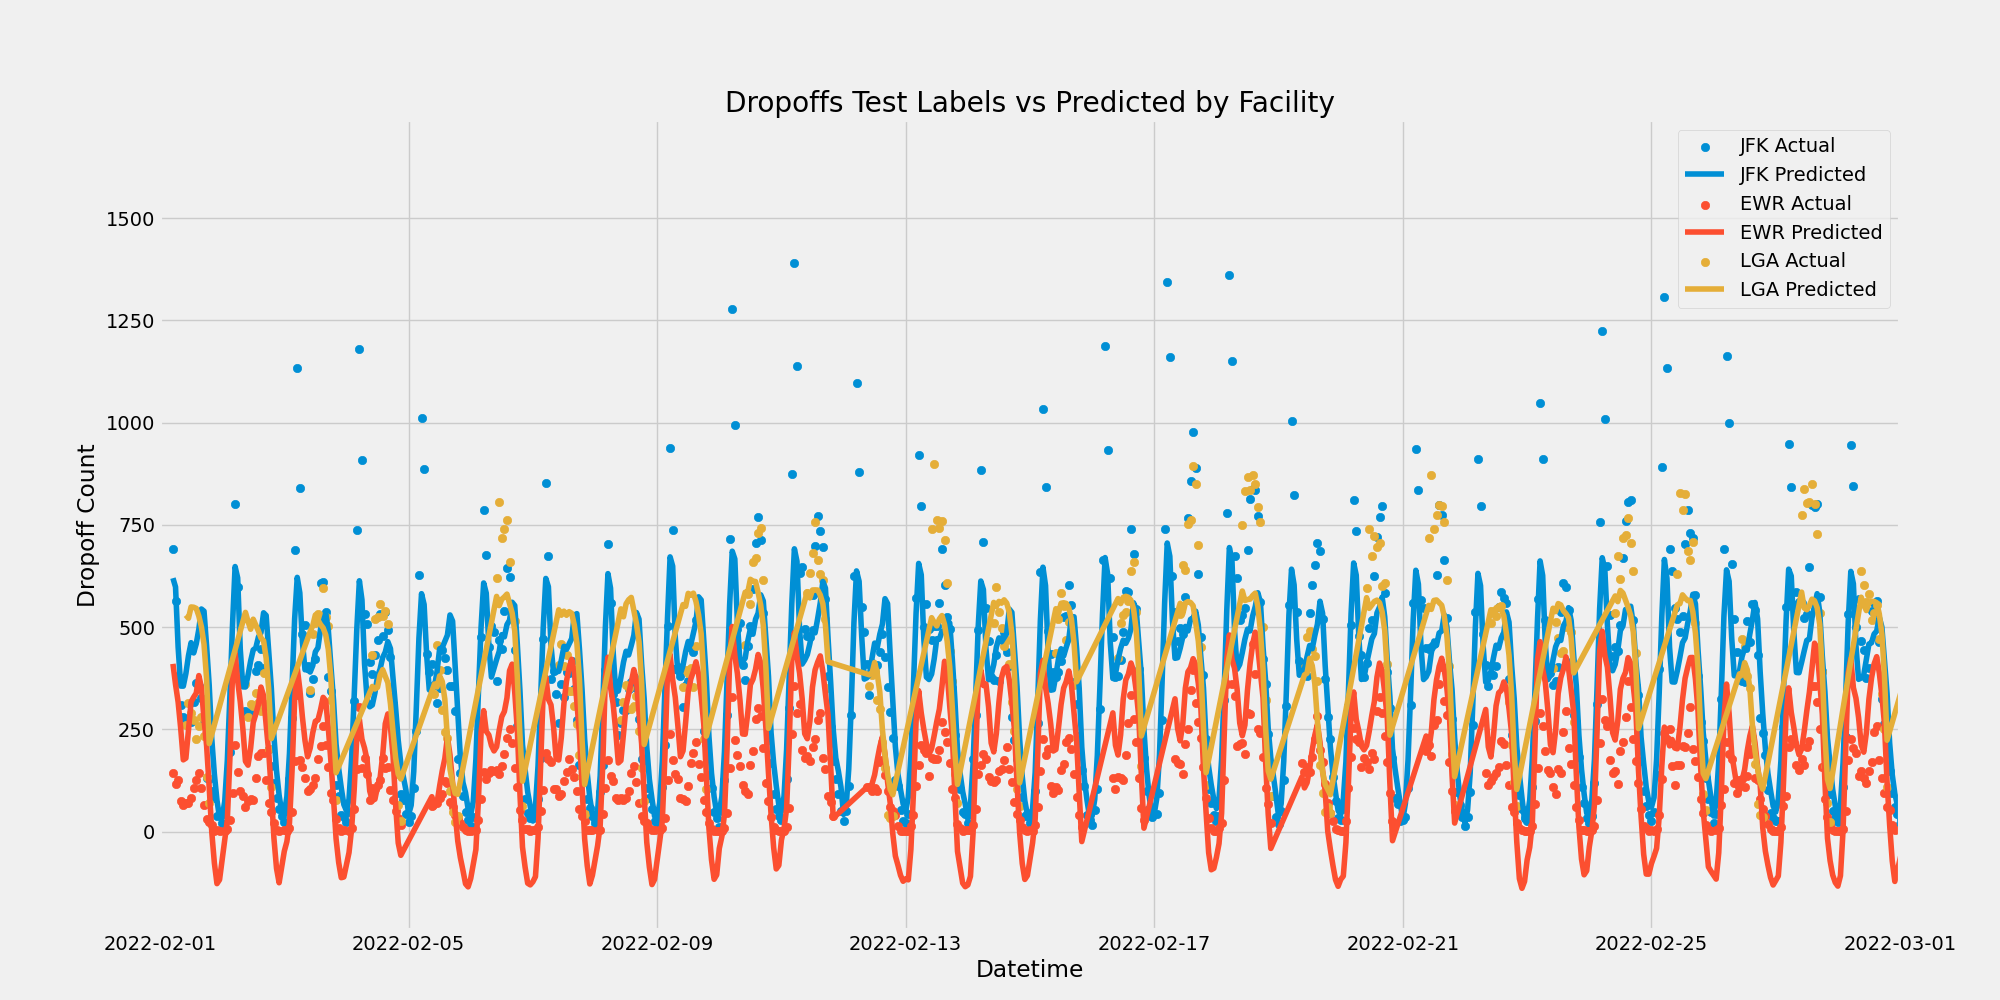
\includegraphics[width=1\textwidth]{plots/Dropoffs Test vs Predicted by Facility.png}
\end{figure}

Clearly, our model does not properly distinguish between the three airports, and tends to underestimate JFK and LGA volumes especially at extreme data points. This is likely because the model does not account for the vast differences in distribution between the airports, and the differences in impact of other factors based on the airport facility. Therefore, next, we will explore a model with interaction to remedy this.


\subsection{Elastic Net Least Squares Regression with Interaction}

As demonstrated by the test evaluation of our model above, and ANOVA analysis \ref{tbl:anova_interaction}, there is evidence of interaction between the categorical variables as well as between continuous variables and categorical variables. Thus, we will generate interaction terms for our second model. Interaction terms will allow us to model the effect of relevant variables on one another. For example, as above there are indicators of interaction between day and facility as well as facility and the other numerical features, meaning that we can evaluate and model the effect of facility on the impact of the other factors in the model. This means that each facility may have a different level/type of impact from arrivals/departures at different points in time, as well as busy days at each airport may differ. We introduce interaction for all pairs of features in order to capture any such relationships, and allow elastic regression to minimise overfitting that may result from overparameterisation.
\begin{figure}[h!]
    \centering
    \caption{Elastic Net with Interaction Pipeline}
    \label{fig:elasticnetinteraction_pipeline}
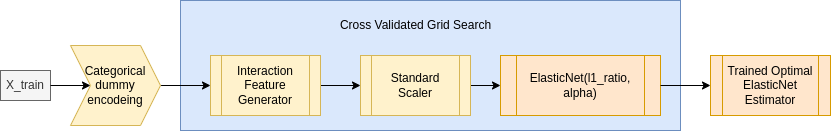
\includegraphics[width=1\textwidth]{plots/elasticnet_pipeline_interaction.png}
\end{figure}


\begin{figure}[H]

\captionof{table}{CV Grid Search Avg. $R^2$ scores across folds for l1 ratio and $\alpha$}
\[
    Pickups
  \begin{array}{cc|ccccc}
    &\multicolumn{1}{c}{} & \multicolumn{5}{c}{\text{l1 ratio}} \\
    && .1 & .5 & .7 & .9 & \textbf{1} \\
    \cline{2-7}
    & \textbf{.1} & .860 & .862 & .864 & .865 & \textbf{.866} \\
    \smash{\rotatebox[origin=c]{90}{\text{$\alpha$}}} & 1 & .829 & .838 & .844 & .852 & .857 \\
    & 10 & .647 & .688 & .717 & .761 & .800
  \end{array}
  \qquad
  Dropoffs
    \begin{array}{cc|ccccc}
    &\multicolumn{1}{c}{} & \multicolumn{5}{c}{\text{l1 ratio}} \\
    && .1 & .5 & .7 & .9 & \textbf{1} \\
    \cline{2-7}
    & \textbf{.1} & .941 & .943 & .944 & .945 & \textbf{.946} \\
    \smash{\rotatebox[origin=c]{90}{\text{$\alpha$}}} & 1 & .907 & .920 & .927 & .934 & .936 \\
    & 10 & .704 & .757 & .796 & .856 & .898
  \end{array}
\]
\end{figure}

An interesting result of our grid search is the choice of 1 as l1 ratio for both datasets. This is likely because generating interaction creates a large number of features, and as such l1 regression is optimal as it ensures that the coefficients are sparse and minimises the number of relevant features to the model, thus preventing any fitting to noise from the vast number of features (which due to interaction may be highly correlated with one another).


\begin{figure}[H]
    \centering
    \caption{Dropoffs Performance Visualisation on a subset of test data by facility with Interaction}
    \label{fig:dropoffsperformanceinteraction}
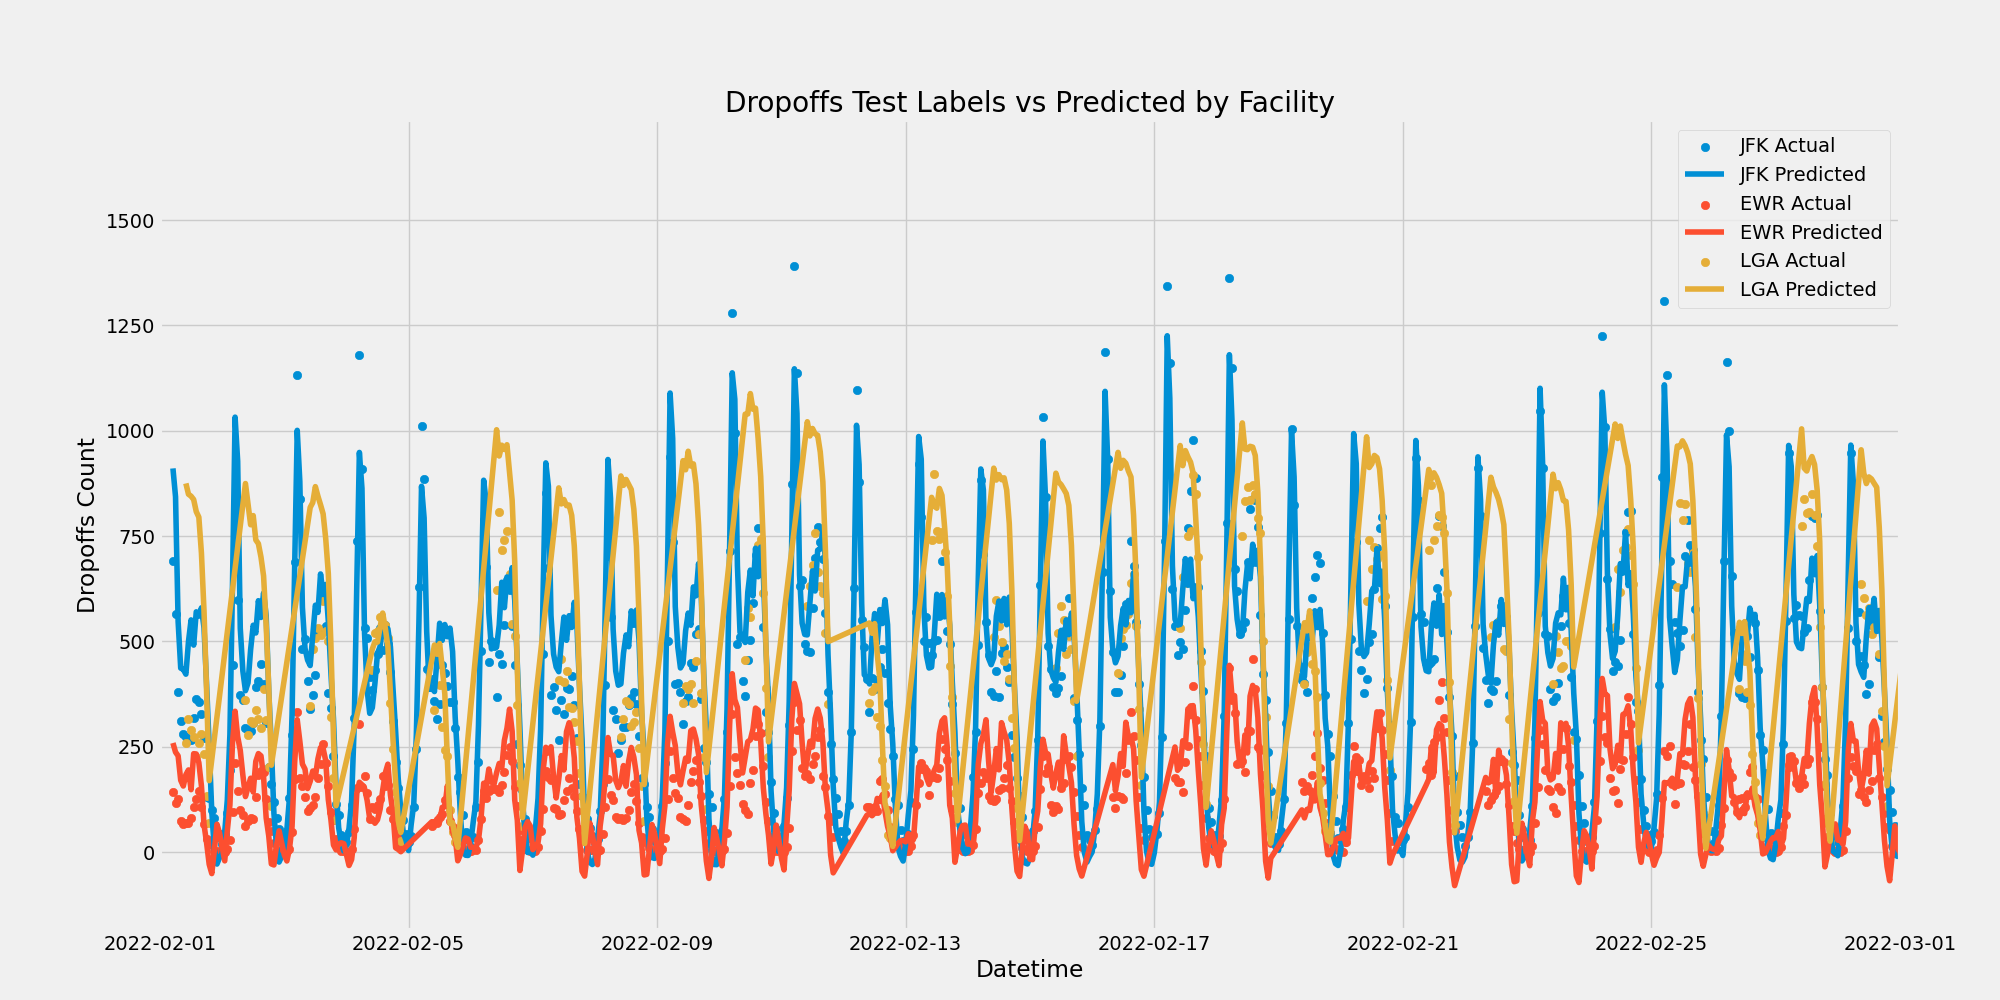
\includegraphics[width=1\textwidth]{plots/Dropoffs Test vs Predicted by Facility with Interaction.png}
\end{figure}


\subsection{Evaluation and Comparison}

In addition to the above plots \ref{fig:dropoffsperformance} \ref{fig:dropoffsperformanceinteraction}, we also evaluate our models using Mean Absolute Error (MAE) and the Coefficient of Determination $R^2$
We select these metrics as they are both quite easily interpretable in the context of our problem. The below are metric outputs from our two models for both datasets, with information on training and testing performance. 
\begin{figure}[H]
    \caption{Model Test \& Train Output Metrics}
    \label{fig:metrics}
    \begin{subfigure}{.5\textwidth}
        \subcaption{Base}
        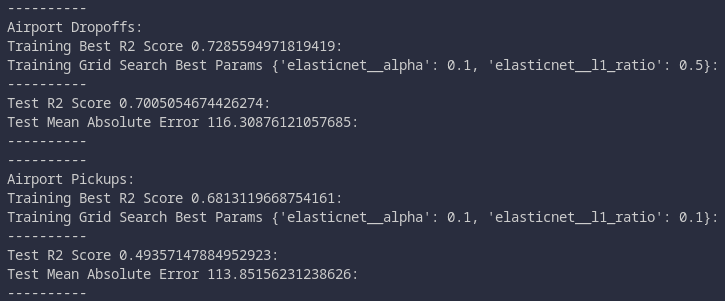
\includegraphics[width=1\textwidth]{plots/output.png}
    \end{subfigure}
    \begin{subfigure}{.5\textwidth}
        \subcaption{Interaction}
        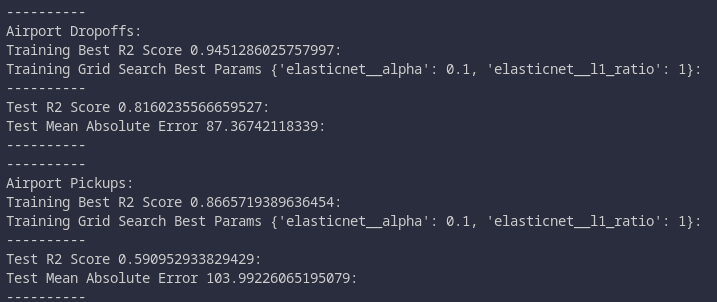
\includegraphics[width=1\textwidth]{plots/Interaction_output.png}
    \end{subfigure}
\end{figure}

As we can see, the interaction model clearly performs much better than the base model. However, it is evident that while the base model generalises well with little overfitting (has much more similar training and test $R^2$), the interaction model experiences a significant dropoff in performance when testing. This is likely because of the introduction of a large number of interaction terms. While a large of these have 0 coefficients (153/253 and 145/253 have non-zero coefficients) thanks to LASSO, there is still a much larger number of factors contributing to noise and thus it is likely that there is a significantly larger amount of overfitting in this model compared to the base model. On the other hand, as demonstrated by our testing in a 2022 dataset, the interaction model still handily outperformed the base model on both metrics, meaning that despite a larger impact of overfitting, the interaction model generalises sufficiently well to perform a better predictive model for our problem. 

More specifically, as per the $R^2$, our interaction model is able to explain 81.6\% and 59.1\% of variance in the test set's response (dropoff and pickup counts respectively) through linear relationships with features in the model compared to the non-interaction model's 70.0\% and 49.4\%. Furthermore, the MAE of the interaction model was 87.4 for the dropoff dataset, meaning that it on average "mis-predicts" dropoff counts by 87.4 units. This is contrasted by the much higher errors from not only the base model (116.3, 113.9 for dropoffs and pickups), but also compared to pickups with interaction. This not only demonstrates that the interaction model is less prone to error than the base model, even when extrapolating, but that the model for the pickup dataset is significantly less robust, more prone to overfitting and significantly less accurate at extrapolating. This is further reinforced by the large disparity in training and test $R^2$ which is only amplified in the interaction model, which is a strong indicator of overfitting. This can likely be attributed to the test distribution deviating significantly from the test distrbution in the given time periods (as the model performs well otherwise, for example on the dropoff dataset). 

\section{Recommendations}
We address the implications of this paper on each of the possible stakeholders identified in the introduction. 
Firstly, for ride sharing services whose data is present in the FHVHV dataset, we have demonstrated a strong relationship between flight arrivals and departures and ride counts, indicating a possible driver of demand for airport pickup/dropoff rides. Therefore, we recommend that ride sharing services incorporate temporally shifted real-time flight data (including flight schedules and history) in their pricing and allocation algorithms in order to maximise profit. This could simply be done by utilising public or private flight APIs to capture flight data and including it as a factor in any surge pricing models used by such services.
Secondly, for ride sharing service drivers, this model may be used as part of either the ride sharing service and/or an external application to predict optimal stand by locations to maximise ride potential. For example, drivers may be notified when indicators of high future dropoff/pickup volume (eg. when a lot of flights are departing or leaving an airport), allowing them to plan their shifts to take on airport faring passengers. This may require additional data to model the origin of airport passengers, in order to utilise the dropoff model to inform optimal ride seeking locations. On the other hand, the pickup model could be used to inform drivers when and which airport to stand by at for maximal ride probability.
Finally, for customers and customer facing businesses (eg. travel agencies), an additional factor to getting the cheapest ticket may be avoiding surge pricing, for example by avoiding high ride volume times for flights to minimise additional transportation costs. For example, a travel agency may use this model to advise passengers to travel during the night, as the lower number of plane arrivals/departures lead to a lower volume of rides and thus a relaxation of surge pricing and a higher availability of rides on landing/departure.

\clearpage

% BEGIN REFERENCES SECTION
\printbibliography

\end{document}